\section{Evidencias del levantamiento y trazabilidad}
\label{anexo:evidencias}

\subsection{Procedencia y organización}

El levantamiento inicial del SGRA se documentó mediante cinco entrevistas, sus grabaciones y las transcripciones del Anexo G del informe original~\cite{SGRA-documentacion-original}. Este material, junto con los consentimientos firmados disponibles, se conserva en \nolinkurl{evidencias/levantamiento/}. El inventario de la carpeta relaciona cada entrevista con su participante, audio, transcripción y respaldo de consentimiento.

Las entrevistas se realizaron en junio de 2025. Los audios y los consentimientos se cargaron en Drive el mismo día de su obtención, por lo que las fechas de carga permiten fechar el levantamiento. Los tres formularios firmados autorizan la grabación de voz y su uso educativo. Aunque la plantilla identifica la pertenencia institucional como alumno, los participantes intervinieron en calidad de docentes, según se describe en el informe original.

\subsection{Entrevistas y respaldo de consentimiento}

\begin{longtable}{@{}p{0.12\textwidth}p{0.30\textwidth}p{0.43\textwidth}@{}}
\toprule
\textbf{ID} & \textbf{Participante y audio} & \textbf{Respaldo recuperado}\\
\midrule
\endhead
ENT-01 & Jessica Ponce, coordinación~\cite{Ponce2025-Entrevista}. & Declaración del equipo sobre el consentimiento para grabar, recogida en la transcripción a los 00:29.\\
ENT-02 & Efraín Díaz, docente~\cite{Daz2025}. & La transcripción recoge la solicitud de permiso a los 00:07 y la respuesta a los 00:13.\\
ENT-03 & Angelita Bosquez, docente en línea~\cite{Bosquez2025}. & Consentimiento firmado para grabación de voz y uso educativo~\cite{consentimiento-bosquez}.\\
ENT-04 & Daisy Nata, docente~\cite{Nata2025}. & Consentimiento firmado para grabación de voz y uso educativo~\cite{consentimiento-nata}.\\
ENT-05 & Carlos Márquez de la Plata, docente~\cite{MarquezdelaPlataMontiel2025}. & Consentimiento firmado para grabación de voz y uso educativo~\cite{consentimiento-plata}.\\
\bottomrule
\end{longtable}

Las cinco transcripciones reproducen íntegramente las entrevistas. Los archivos originales y sus enlaces se encuentran en el inventario local y en las referencias.

\subsection{Localizadores y trazabilidad hacia los requisitos}

Las cinco transcripciones se incluyen en el Anexo~\ref{anexo:transcripciones}, organizadas por participante y vinculadas con los identificadores ENT-01 a ENT-05. Las entrevistas de coordinación, Efraín Díaz y Carlos Márquez de la Plata contienen marcas de tiempo; las de Angelita Bosquez y Daisy Nata están organizadas en preguntas y respuestas sin esas marcas. La entrevista de coordinación sustenta los hallazgos H-01 a H-05 de la Tabla~\ref{tab:trazabilidad-contexto}.

La Tabla~\ref{tab:anexo-origen-rf} relaciona los quince requisitos funcionales con las entrevistas, el catálogo, las reglas de proceso y las historias del SGRA original~\cite{SGRA-documentacion-original}. Las páginas corresponden a la numeración impresa de ese informe. Los criterios de aceptación se presentan en la Tabla~\ref{tab:trazabilidad-rf}.

El análisis funcional del equipo complementó las necesidades expresadas en las entrevistas con reglas para completar los procesos, mantener la coherencia de los estados y delimitar los permisos de cada rol. La trazabilidad identifica tanto los hallazgos de entrevista como los requisitos derivados de ese análisis y sus ajustes al alcance del PFC. Para ENT-03 y ENT-04, las preguntas sirven como localizadores de los pasajes que carecen de marcas de tiempo.

\begingroup
\small
\setstretch{1.05}
\begin{longtable}{@{}p{0.08\textwidth}p{0.35\textwidth}p{0.49\textwidth}@{}}
\caption{Origen y hallazgo de los requisitos funcionales de E1}
\label{tab:anexo-origen-rf}\\
\toprule
\textbf{RF} & \textbf{Entrevista o fuente original} & \textbf{Hallazgo y delimitación actual}\\
\midrule
\endfirsthead
\toprule
\textbf{RF} & \textbf{Entrevista o fuente original} & \textbf{Hallazgo y delimitación actual}\\
\midrule
\endhead
RF01 & ENT-01, 07:54 y 11:28 (G.1, p. 166); RF03--RF04, RP01 y HU-01 (pp. 77--78, 90, 194--195). & H-03 y H-04: atención individual o grupal ligada a asignaturas activas. El motivo, adjunto y selección de compañeros proceden del análisis previo. El análisis del registro incorpora el aviso inmediato cuando falta un docente asignado y la preferencia horaria del estudiante.\\
RF02 & ENT-01, 13:24 (G.1, p. 166); RF06 y HU-02 (pp. 78, 195). & H-05: el estudiante necesita información de su tutoría. El análisis funcional define los estados y filtros de consulta. El acceso a grupales se realiza desde la cuenta propia.\\
RF03 & Derivado del análisis funcional: RF07 y HU-02 (pp. 78, 195). & El análisis previo permite cancelar solicitudes pendientes. Se precisa que, en una grupal, solo el estudiante creador puede cancelarla; los demás participantes pueden consultarla.\\
RF04 & ENT-01, 13:24 (G.1, p. 166); RF08, RP03 y HU-02 (pp. 78, 90, 195). & H-05: conocer lugar, hora y modalidad. Los campos del detalle y la visualización del enlace proceden del análisis funcional. Se distingue lo programado de los datos aún pendientes.\\
RF05 & ENT-02, 14:04--14:13 (G.1, p. 167); RF09 y HU-02 (pp. 78, 195). & Conservar evidencia de las sesiones. La entrevista respalda esa necesidad general; el historial del estudiante, los filtros y la descarga de recursos se especificaron en el análisis previo.\\
RF06 & ENT-02, 08:41--08:56 (G.1, p. 167); RF10 y RP02 (pp. 78--79, 90). & El docente necesita aceptar o rechazar solicitudes. La asignación, el estado pendiente y el motivo opcional se concretan mediante los requisitos y el proceso previos.\\
RF07 & ENT-02, 01:26--02:23, 09:14--10:40 y 12:39--13:15 (G.1, p. 167); ENT-04, pregunta sobre dificultades (pp. 169--170). RF11--RF13 y RP03 (pp. 79, 90). & Se necesitan modalidad, disponibilidad y duración configurable; ENT-04 advierte choques de horario. El proceso de reserva concreta el tipo Aula o Laboratorio y su envío al gestor.\\
RF08 & ENT-02, 08:41--08:56 (G.1, p. 167); RP04 (p. 90). & El docente necesita reprogramar la atención. El análisis del proceso define los estados habilitados, la validación del espacio y las respuestas al nuevo horario.\\
RF09 & ENT-02, 16:45--17:04 (G.1, p. 168); RF15 (p. 79). & Registrar asistencia o, al menos, participantes. La asistencia de una sesión reprogramada se limita a quienes aceptaron el horario vigente, de acuerdo con RF15.\\
RF10 & ENT-02, 14:04--14:13 (G.1, p. 167); RF16 (p. 79). & Conservar evidencia del trabajo realizado. Observaciones, resultados, cierre y recursos provienen del requisito anterior; el cierre de una sesión reprogramada requiere al menos una aceptación del horario vigente.\\
RF11 & ENT-01, 00:51 y 01:16 (G.1, p. 165); RF29--RF30, RP08 y HU-05 (pp. 81, 91, 197--198). & Coordinación supervisa el cumplimiento y el rendimiento. El alcance del PFC concentra este rol en el seguimiento de solo lectura, con los datos académicos provistos por el SGA.\\
RF12 & ENT-02, 01:37--02:20 (G.1, p. 167); RF13, RF18--RF20, RP03 y HU-04 (pp. 79--80, 90, 196). & La falta de laboratorios dificulta la atención presencial. El gestor y las reservas se detallaron en el análisis previo. El proceso contempla sesiones individuales y grupales, motivo opcional de rechazo y acciones diferenciadas de reasignación de espacio y cancelación del refuerzo.\\
RF13 & Derivado del análisis funcional: RF24--RF28, RF30, RF33--RF35 y HU-06 (pp. 80--82, 198--199). & Administración de cuentas, permisos, parámetros, auditoría, respaldos, correo e identidad visual, procedente del análisis funcional. RF13.1--RF13.6 desglosan esas obligaciones; se limita la escritura a datos locales del SGRA.\\
RF14 & ENT-01, 06:44 y 13:24 (G.1, p. 166); ENT-03, pregunta sobre notificaciones (p. 168); ENT-04, pregunta sobre el medio de notificación (p. 170). RF31, RP09 y HU-07 (pp. 81, 91, 199). & H-02 y H-05: avisos oportunos con información de la sesión. ENT-03 y ENT-04 prefieren correo. El análisis funcional concreta el envío mediante Gmail, la notificación de cada cambio de estado y el registro de fallos de envío.\\
RF15 & ENT-02, 08:41--08:56, solo como contexto de reprogramación (G.1, p. 167). RP04 y RP06 (pp. 90--91), como antecedentes. & El análisis del flujo de reprogramación incorpora la respuesta individual al nuevo horario para respetar la disponibilidad de cada participante. Una aceptación permite continuar la sesión. Si todos rechazan, se rechaza el refuerzo completo. RP04 y RP06 aportan los antecedentes de reprogramación y participación grupal.\\
\bottomrule
\end{longtable}
\endgroup

\subsubsection{Fechas de las entrevistas}

Las fechas de las entrevistas corresponden al registro de carga de los audios en Drive, realizado el mismo día de cada sesión:
\begin{itemize}
\item ENT-01, Jessica Ponce: 27 de junio de 2025.
\item ENT-02, Efraín Díaz: 29 de junio de 2025.
\item ENT-03, Angelita Bosquez: 28 de junio de 2025.
\item ENT-04, Daisy Nata: 29 de junio de 2025.
\item ENT-05, Carlos Márquez de la Plata: 28 de junio de 2025.
\end{itemize}
Los consentimientos firmados se conservan junto con las grabaciones como respaldo de la autorización para su uso educativo.


\subsection{Encuesta y validaciones del sistema anterior}

Se conserva el enlace al panel de resultados de la encuesta estudiantil~\cite{Toaquiza2025}. El Anexo G.2 informa de 21 participantes. El panel y los resultados resumidos documentan este antecedente; la exportación de las respuestas individuales está pendiente de recuperación.

Las conversaciones de validación posteriores se mantienen como evidencia complementaria en su carpeta de Drive~\cite{Ponce2025-Validacion}. Su inventario comprende las grabaciones de Efraín Díaz, la licenciada Arrata, Daisy Nata y la Product Owner. La referencia aportada sitúa las conversaciones en julio de 2025; las fechas de carga de los archivos varían y requieren distinguirse de las fechas de sesión.

\subsection{Evidencia fotográfica referencial}

La Figura~\ref{fig:validacion-previa} se incorpora como evidencia referencial del trabajo presencial con los interesados durante el desarrollo del SGRA~\cite{SGRA-documentacion-original}.

\begin{figure}[htbp]
\centering
\IfFileExists{evidencias/levantamiento/fotografias/validacion-previa-000.jpg}{%
  \includegraphics[width=0.44\textwidth]{evidencias/levantamiento/fotografias/validacion-previa-000.jpg}%
}{%
  \includegraphics[width=0.44\textwidth]{../evidencias/levantamiento/fotografias/validacion-previa-000.jpg}%
}
\caption{Evidencia referencial del trabajo presencial con los interesados del SGRA.}
\label{fig:validacion-previa}
\end{figure}
